\section{Design}
\label{sec:DesignImplementation}
\vspace{\baselineskip}
\subsection{Development Process} 
\par 
\vspace{\baselineskip}
\hspace{1em}
The basic concept and outcome of the PAMEx project was well defined 
from the beginning, but there were several unknowns about how to 
achieve several goals. It was also decided early on that the project 
would need to be broken into several segments to achieve what was 
necessary but also to allow a privileged user of PAMEx to have the 
customizability to implement PAMEx on different systems effectively 
and isolate the different processes of the security system. Therefore, 
the project implementation would need to be flexible, but efficient 
and would need to be treated as several tools working together to 
achieve a desired end state. Once fully designed, PAMEx would become a tool 
suite with several components including a customized compiler, a file 
labeler and user database builder, a PAM module, the Oracle tool for 
determining a user’s access to a file, and an extraneous file labeler 
to make retrospective file labeling easier. With all these factors in 
mind, it was decided that an Agile approach was the best implementation 
strategy for this project and that using the Scrum framework was the 
best way to achieve this. Agile is a model which focuses on an incremental approach to 
programming by developing a working product in iterations rather than all at once \cite{kung2014}. 
In addition, the Agile method via a Scrum 
framework is immensely popular among many industries \cite{lacey2015} and therefore, 
Agile and Scrum were valuable skills to research 
alongside the development of the project. 

Two sources were researched and followed as guidelines for the 
Scrum process throughout the project. The first source 
acted as an introduction to the Scrum process and is a blog entitled 
“What is Scrum?” on the official Scrum website \cite{scrumorg}. The second 
source is a book entitled “The Scrum Field Guide” authored by 
Mitch Lacey, which acted as an ongoing guide \cite{lacey2015}. In the first source it was found that Scrum is a cyclical process in which there are groups of 
individuals that work to achieve a common goal. Figure~\ref{Scrum Diagram}
was taken from the first source and depicts a typical Scrum cycle. Each cycle is referred to as a sprint 
and during each sprint, it is expected that four events occur: first, 
the product owner divides up a complex problem and puts the divided 
pieces into a backlog, second, the Scrum team creates an incremental 
product, third, the Scrum team inspects the results and adjusts for 
the next sprint, and fourth, the process is repeated \cite{scrumorg}.
\clearpage

\begin{figure}[h]
\centering
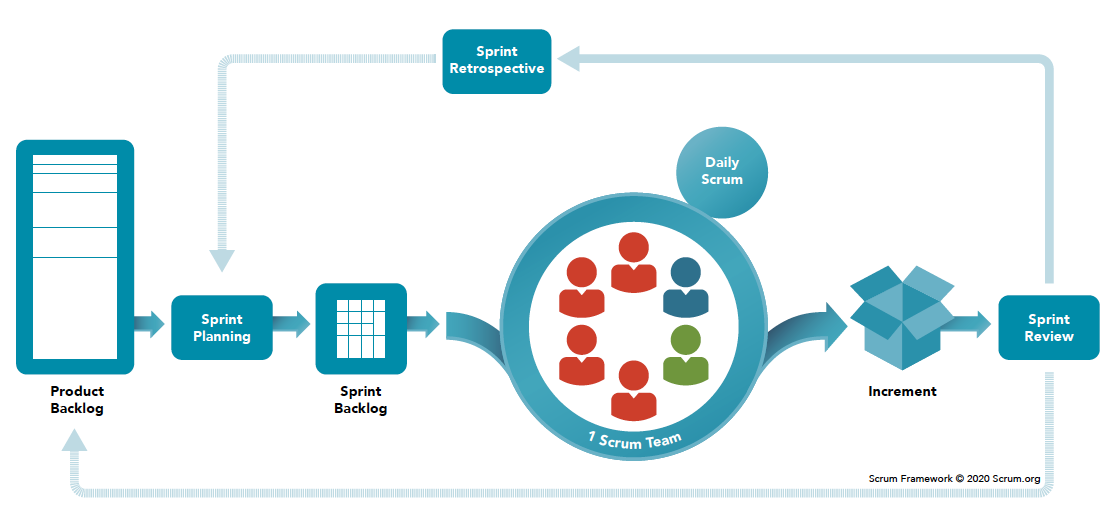
\includegraphics[width=.8\textwidth]{section03/assets/scrum-cycle.png}
\caption[Scrum Cycle Diagram]{\label{Scrum Diagram}A Typical Scrum Cycle (from \cite{scrumorg})}
\end{figure}

\vspace{\baselineskip}

Typically, in a software project setting, the Scrum team is divided 
into three groups: the Scrum master, the product owner, and the 
developers. The Scrum master’s primary job is to help the team focus 
on creating a high-value product increment and remove anything that 
may impede this process. The product owner’s primary job is to 
prioritize the work of the developers. The developers’ job is to 
work on completing the product increment for each sprint. The idea is 
that the Scrum team has all the skills needed to complete the task 
given, and each member is an expert at contributing to at least one of 
the aspects of the project \cite{scrumorg}. 

At the beginning of each sprint, the product owner’s job is to perform 
backlog grooming which means that they determine which parts of the 
product should be completed next and how much development should get 
done for that particular sprint. For each sprint, the team is expected 
to meet regularly for what is known as a standup where they talk about 
the progress that has been made on the product increment and any 
impediments that they have. At the end of a sprint, the team has a 
retrospective meeting where they talk about the previous sprint: both 
what went well and what could be improved \cite{scrumorg}. 

The PAMEx team only consisted of two members and as such, some modifications needed to be made to the Scrum 
process. The Scrum role of the product owner was filled by the author’s 
advisor and the role of the developer was filled by the author; the 
author also filled the role of Scrum master by leading each of the 
standup meetings. Each sprint was decided to be two weeks long, and 
during that time, the Scrum team would meet once per two 
weeks instead of performing a daily standup together. This decision 
was made primarily due to the schedule of both parties and nature 
of the project. The project team only consisting of two members 
led to more direct communication than a typical industry software 
product would. The Scrum team members both had times when communication 
needed to occur before the scheduled sprint time such as for a 
modification in an aspect of PAMEx’s design or if the developer had a 
blocker during development. For these instances, often the team found it sufficient to perform communication via email but 
occasionally set up an online conference call.  

For each biweekly meeting, the team followed Scrum procedure and would perform a standup by 
talking about what was completed during the sprint \cite{lacey2015} and talk 
about any blockers that were present in the current incrementation. Part of the standup 
process included presenting research findings on the 
Scrum process as well. After the standup, the team would 
perform a retrospective and talk about what went well and what needed 
to improve for the next sprint. Finally, the team would 
talk at a high level about what should be completed for the upcoming 
sprint. 

The team chose to track this information with the tool Jira. Within 
Jira, the developer, acting also as the Scrum master divided the functionality requirements of the project 
into Jira tickets. The tickets contained information about each piece of 
the project including the ticket number, the ticket type such as user 
story, sprint task, enhancement, or bug, a description of the ticket 
which often included a definition of done for each stage of the ticket, 
the estimated story points, the amount of development time spent on the 
ticket, the start date, the end date, the priority of the ticket, and 
the relationship that the ticket has to other tickets. Dividing the project
in this way is common when using the Scrum approach so that a team can
easily see what is the next highest priority in the development process to 
complete the next iteration of the product \cite{lacey2015}.

Throughout the project, a total of 35 Jira tickets were created 
with a total of 103 estimated story points in 15 sprints. That equates 
to an average of 6.87 points per sprint or roughly one point every two 
days. Figure~\ref{Points Remaining Diagram} is a chart depicting the amount of total user stories 
remaining to complete compared to the date of the ticket’s 
completion. 

\begin{figure}[h]
\centering
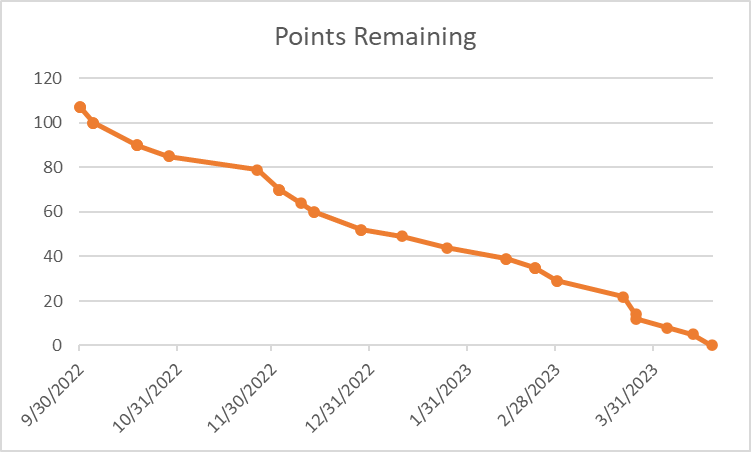
\includegraphics[width=.8\textwidth]{section03/assets/jira-points.png}
\caption[User Story Points Remaining Compared to Date Diagram]{\label{Points Remaining Diagram}User Story Points Remaining Compared to Date}
\end{figure}

\vspace{\baselineskip}

It is easy to tell from the diagram above that there is a steep downgrade toward the end of 
the project, depicting that a lot of user story points were completed 
near the end. This is partially because a 
few large user stories and tasks were designed to be completed at 
the end of the project. Some of these tasks included creating 
documentation for the PAMEx tool and writing a formal manuscript for 
the tool.  

In a Scrum setting, after each sprint, the team should have developed 
and produced an incremental cohesive product. Even if the incremental 
product does not have all of the functionality of the completed product, it should be usable \cite{scrumorg}. 
PAMEx's natural separation yet cohesiveness of different tools made 
it easy to use the incremental approach, so often each sprint was dedicated to the development of a separate PAMEx tool. 
There was not such a natural separation for every sprint however, 
as some of the aspects of the project, for example the compiler, were 
much bigger than others. Therefore, incremental, 
cohesive parts of the larger pieces were developed separately. 
To continue with the example of the compiler, the compiler was divided into five separate sprints and therefore 
into five different components. The components included 
defining the syntax and grammar for the policy including creating a 
prototype EBNF diagram, creating the Flex lexer, creating the Bison 
parser, and two components for implementing the semantic functions that 
would be triggered by the grammatical parser. The separation of the semantic functions occurred 
naturally because the grammar already essentially had an informal 
separation: definition statements and assignment statements. Therefore, 
during the first of these two sprints, the 
semantic functions pertaining to the grammar that defined security 
levels and labels were developed, and the during the second, 
developing the semantic functions pertaining to the grammar that 
assigned the security levels and labels to users and files was focused on. 

During each day of a sprint, more aspects of the Scrum 
process were practiced. For each day of development, the product’s ticket board which 
included the product backlog would be viewed and updated. 
This served as a replacement for the daily standup that would have 
otherwise been performed. For each user story, a 
definition of done was created for each of the stages of development. The stages 
included the development process, the review process in which the 
product increment was reviewed by the product owner/advisor, and the 
testing process. It was found that a definition of done is an 
integral part of the Scrum process as it defines when each user story 
is completed \cite{lacey2015}\cite{scrumorg}. 

Although the Scrum process 
had been modified, the spirit of Agile development via the Scrum method was kept and 
the core principles were still followed during the development of PAMEx. In doing so, the PAMEx project was 
able to be developed at a manageable, incremental pace to focus on each aspect of the project independently. 
\vspace{\baselineskip}

\subsection{Technologies}
\par 
\vspace{\baselineskip}
\hspace{1em}
All components of the PAMEx tool suite were developed in Vim or Visual 
Studio Code using the programming languages C, Flex, and Bison. 
C was chosen as the primary language for the 
development of PAMEx for several reasons. A major reason is that 
SimpleFlow, the project for which PAMEx was designed to enhance was 
built using C \cite{ryan2016} and therefore, it would be easier to integrate PAMEx into the 
SimpleFlow system. Secondly, PAMEx was designed to be tailored to Linux 
security systems. The C programming language has several libraries to 
be able to achieve this. While not all 
aspects of the Linux security system that were needed to be developed for PAMEx were fully understood at 
the beginning of the project, it was known that the security system 
tools that were being sought out to develop could be created using C \cite{linuxpam}\cite{man7pam}\cite{man7xattr}\cite{selinux}. 
Third, from the first design of the PAMEx system, it was known that a custom compiler would be created. 
This is a process that was familiar to the developer using the C language with Flex and Bison. 
\vspace{\baselineskip}

\subsection{PAMEx Design Overview} 
\par 
\vspace{\baselineskip}
\hspace{1em}
The basic flow of PAMEx was designed as follows. First, a 
privileged user writes a PAMEx language file. The PAMEx parser takes 
this file as input and produces two text files as output: one which 
contains a database of the levels defined in the input file and their 
corresponding placements in the level hierarchy, and one which contains 
file and user definitions in a format that is readable by the File 
Labeler and User Database Builder (FLUDB). The definitions file is then 
read by the FLUDB line by line. From this file, the FLUDB can write 
extended attributes attached to the targeted files as metadata. The 
extended attributes will then contain the security information 
specified in the PAMEx language file including both levels and labels. 
The FLUDB tool also creates a text file that acts as a targeted users 
database, containing all the users defined in the PAMEx language file 
and their security information. It is assumed by PAMEx's PAM module that when a user logs in 
to a system that has PAMEx installed on it, the system will have a 
targeted users database file on the system for the kernel to read and 
interpret. Upon a user logging into such a system, the system can 
trigger the custom-made PAM module to write the user clearance 
information to the currently running process. Any action then 
performed by the logged-in user will be branched from the currently 
running process and will therefore contain the user’s clearance 
information \cite{linuxpam}. All that a kernel would need to do when a user tries to 
access a file is cross-check the currently running process’ user 
security information with the file’s security information via extended 
attributes to ensure that a user has the correct clearance level and 
labels and allow the user to export the information from files that 
they have access to. This flow is depicted by Figure~\ref{Capstone High Level Diagram} below.
\clearpage

\begin{figure}[h]
\centering
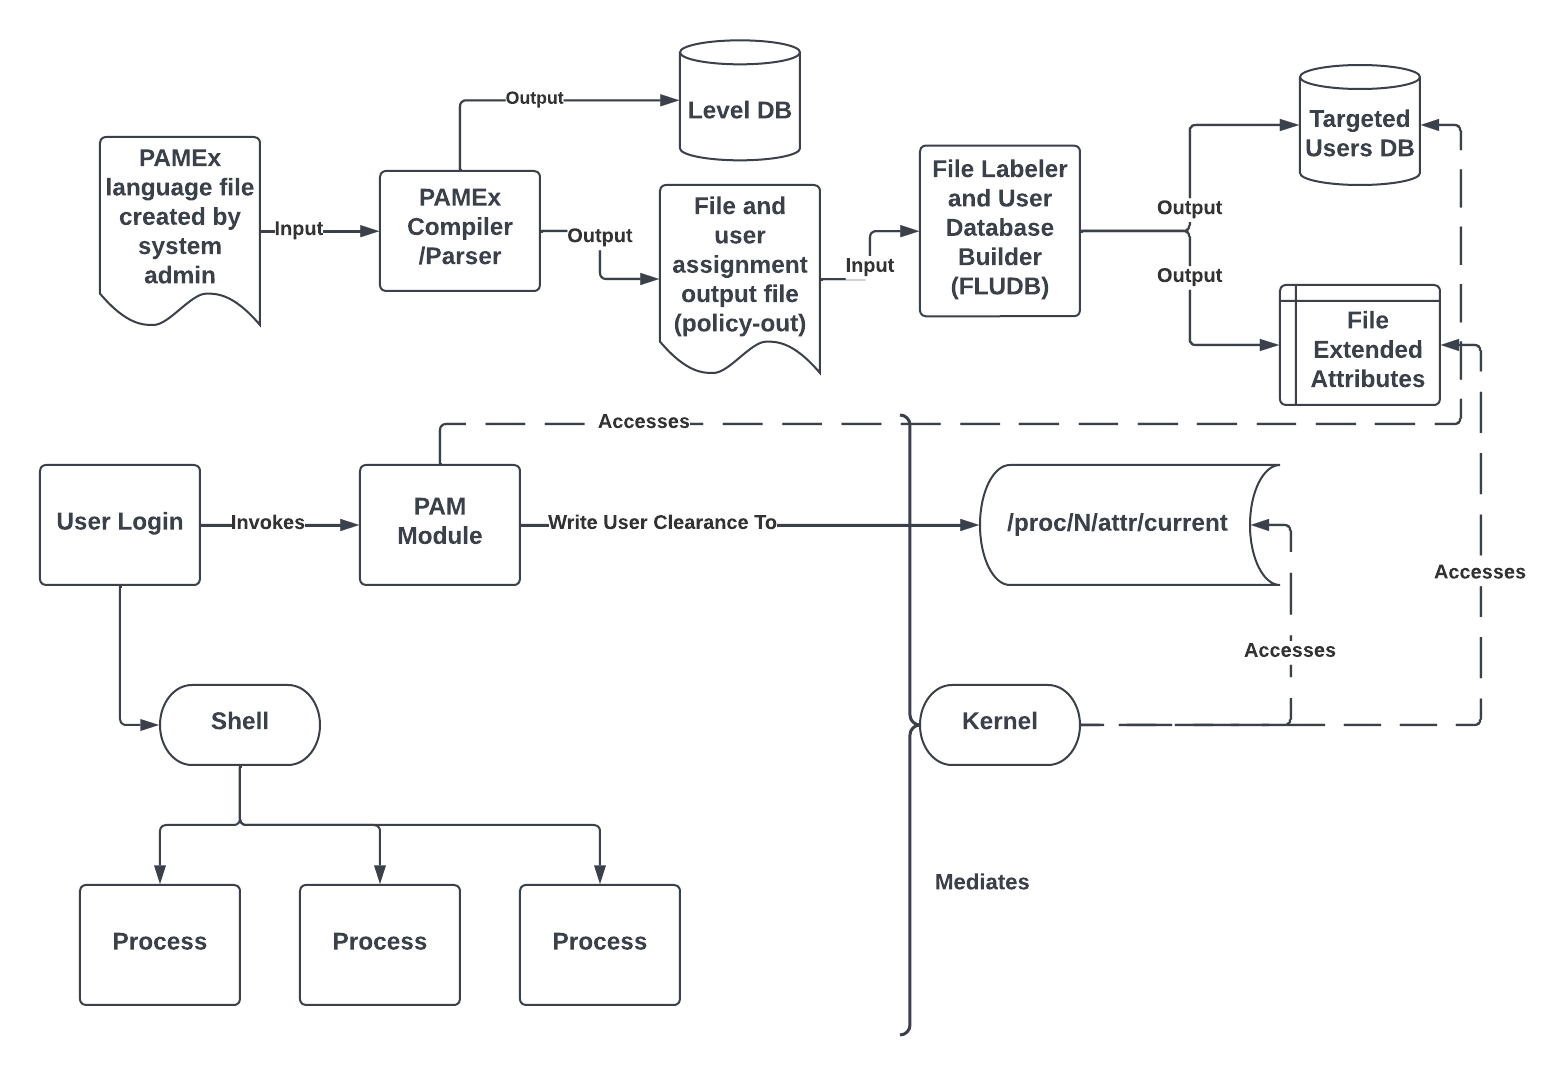
\includegraphics[width=\textwidth]{section03/assets/capstone-high-level.png}
\caption[PAMEx High Level Flowchart]{\label{Capstone High Level Diagram}PAMEx Depicted at a High Level}
\end{figure}

\vspace{\baselineskip}

The original design for the PAMEx project consisted of the compiler, a 
C tool to interpret the compiler’s output, an unknown way for the file 
information to be stored on the system, and a PAM module to collect and 
persist the logged in user’s information. It was known early on that 
enforcing a security policy defined by PAMEx would require a custom 
kernel module. When the project first began, it was intended to also build this kernel module, but as the 
development continued, it was decided that much of the 
security policy functionality would be in place without the kernel and PAMEx’s functionality 
could be demonstrated without it by simulating the kernel's primary 
functionality with a custom-built tool called Oracle.  

The implementation of the PAMEx tool suite followed a path similar to 
the cycle of the implementation of a security policy on a PAMEx system. 
It began first with the compiler by using Flex for the complier’s lexer 
and Bison for the compiler’s grammatical parser. Along with the parser, 
the symbol table was implemented to keep track of the different usages 
of variables and their data types \cite{levine2009}. In the first stage of the compiler’s 
implementation, a level database was not created as a biproduct of the 
compiler’s output because the issue that the level database would later 
solve of ensuring that there was only one set of levels on a system and 
that they were all to be checked by one source was not foreseen yet. 
This would change near the end of PAMEx’s development during the creation 
of Oracle. 

Following the implementation of the compiler, research was done 
to find that the way that many Linux security modules label files with 
security information is through the use of extended attributes \cite{selinux}. 
Extended attributes were found to be accessible through both command 
line processes and using a C library. The complier output interpreter 
tool was therefore created whose job it was to output the PAMEx policy 
assignment information. The file was later renamed to the File Labeler 
and User Database Builder or FLUDB to better describe the functionality 
of the tool.  

The PAM module was then researched and created using the 
Official PAM Modules as a reference \cite{linuxpam}. It was decided to implement 
PAMEx’s PAM module on a virtual machine to not interfere with and 
possibly break the login process of a real system. 

Research was done to grow an understanding of the complexity of 
creating a custom Linux kernel in comparison to the amount of 
functionality that it would be able to demonstrate \cite{kerneldocs}. As a result, 
the informed decision was made to not develop a custom kernel for 
PAMEx and to instead simulate the PAMEx tool suite using another 
custom-developed C tool named Oracle. With Oracle in place, PAMEx as a 
working tool suite could be fully demonstrated from end-to-end. 
\vspace{\baselineskip}
